\documentclass[11pt, fleqn, titlepage]{article}

\documentclass[11pt, fleqn]{article}

\usepackage[usenames,dvipsnames,svgnames,table]{xcolor}
\usepackage{amsmath}
\usepackage{amsfonts}
\usepackage[margin=1in]{geometry} % To set the margin widths
\usepackage{graphicx}
\usepackage{listings}
\usepackage{multirow}
\usepackage{tabularx}
\usepackage{varioref}
\usepackage[noabbrev,capitalize]{cleveref}
\usepackage[group-separator={,}]{siunitx}
\usepackage{subcaption}
\usepackage{titlesec}
\usepackage{lscape}
\usepackage{bm}
\usepackage[titletoc,toc,title]{appendix}

\lstset{
  frame=single,
  basicstyle=\ttfamily,% print whole listing small
  language=R,
  aboveskip=3mm,
  belowskip=3mm,
  showstringspaces=false,
  columns=flexible,
  numbers=none,
  commentstyle=\color{ForestGreen},
  stringstyle=\color{Maroon},
  breaklines=true,
  breakatwhitespace=true,
  tabsize=2,
  literate={<-}{{$\gets$}}1 {~}{{$\sim$}}1
}

\sisetup{output-exponent-marker=\textsc{e}}

\setlength{\parskip}{12pt} % Sets a blank line in between paragraphs
\setlength\parindent{0pt} % Sets the indent for each paragraph to zero

% \crefname{figure}{Figure}{Figures}
% \crefname{section}{Section}{Sections}
% \crefname{table}{Table}{Tables}
% \crefname{lstlisting}{Listing}{Listings}

\setlength{\parskip}{12pt} % Sets a blank line in between paragraphs
\setlength\parindent{0pt} % Sets the indent for each paragraph to zero

\begin{document}

\title{Machine Learning () HW \#1}
\author{Will Clark \& Matthew DeLio \\
University of Chicago Booth School of Business}
\date{\today}
\maketitle

% Describe the data, show a plot of mileage vs price

\section{Data Description}

The data set for this exercise the sale price and observed mileage for 1000 used cars. We can see in \cref{fig:linear} that the expected inverse relationship between mileage and sale price is borne out by the data (i.e. high-mileage cars are less expensive than low-mileage cars).

\section{Linear Regression Model}

To describe this data, we first estimate a linear model of mileage on price:
\[ p_i = \alpha + \beta m_i + \varepsilon_i \]
where \(p_i\) is the price of car \(i\), \(m_i\) is the observed mileage on car \(i\), \(\alpha\) and \(\beta\) are estimated regression coefficients, and \(\varepsilon_i\) is the residual. We fit a generalized linear model to the data and find that \(\alpha=56359.7\) and \(\beta=-0.35\). That is, a hypothetical used car with no miles would sell for about \$56 thousand, and each additional mile driven lowers a car's expected selling price by \$0.35.

As depicted in \cref{fig:linear}, this model appears to be a weak fit for the data. The distribution of residuals is not normally distributed. The model tends to systematically under-value cars with very low mileage and with very high mileage (see \cref{fig:lin_errors} in the Appendix). 

\begin{figure}[!htb]
  \centering
  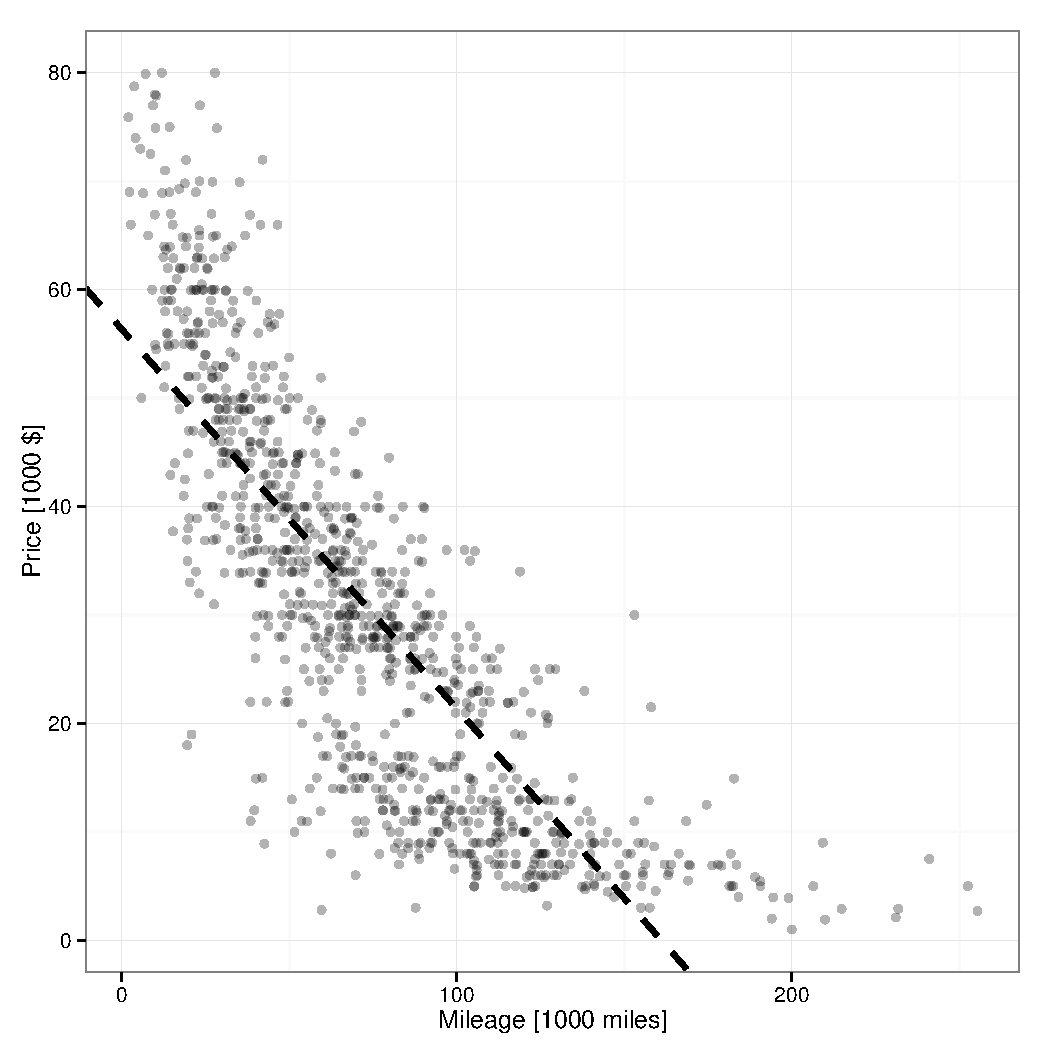
\includegraphics[scale=.5]{linear_fit.pdf}
  \caption{Linear Regression of Price on Mileage}
  \label{fig:linear}
\end{figure}

\section{k-Nearest Neighbors Algorithm}

As an alternative to a linear model, we can use a k-nearest neighbors (knn) algorithm. This algorithm will compute an expected price for every given mileage by taking an average of the observed price for the k-number of cars with the closest observed mileage. 

The decision we are faced with is choosing a value for the k-number of nearest neighbors to include in the algorithm. There are many different decision criteria we could use, but we will focus on two: 1) out-of-sample root mean square error (RMSE); and 2) n-fold cross-validation (CV).

\subsection{Out-of-Sample RMSE}

To choose \(k\) using out-of-sample RMSE, we break our data into a training sample (with 900 data points) to train a model, and a test sample (with the remaining 100 points) to estimate the model's goodness of fit. We then estimate a model for all values of \(k \in (2,100)\) and compare their out-of-sample RMSEs, where RMSE is defined by:
\[ \text{RMSE} = \sqrt{\frac{1}{n} \sum_{i=1}^{n} \left( p_i - \hat{p_i} \right)^2} \]

where \(p_i\) is the observed price of car \(i\) and \(\hat{p_i}\) is the predicted price of car \(i\) given its mileage. The RMSE is a measure of how closely a model fits the data; in this case, what we care about is how well the model fits data points that it has not been trained on. We then choose \(k\) that produces the lowest out-of-sample RMSE. The results are depicted in \cref{fig:sweep} (in the red line). We can see that the minimum RMSE occurs at \(k=11\), which is circled on the plot.

% use n-fold cross-validation
\subsection{n-fold Cross Validation}

The alternative method is to choose \(k\) via cross validation. In this method, we will measure out-of-sample fit 

\begin{figure}[!htb]
  \centering
  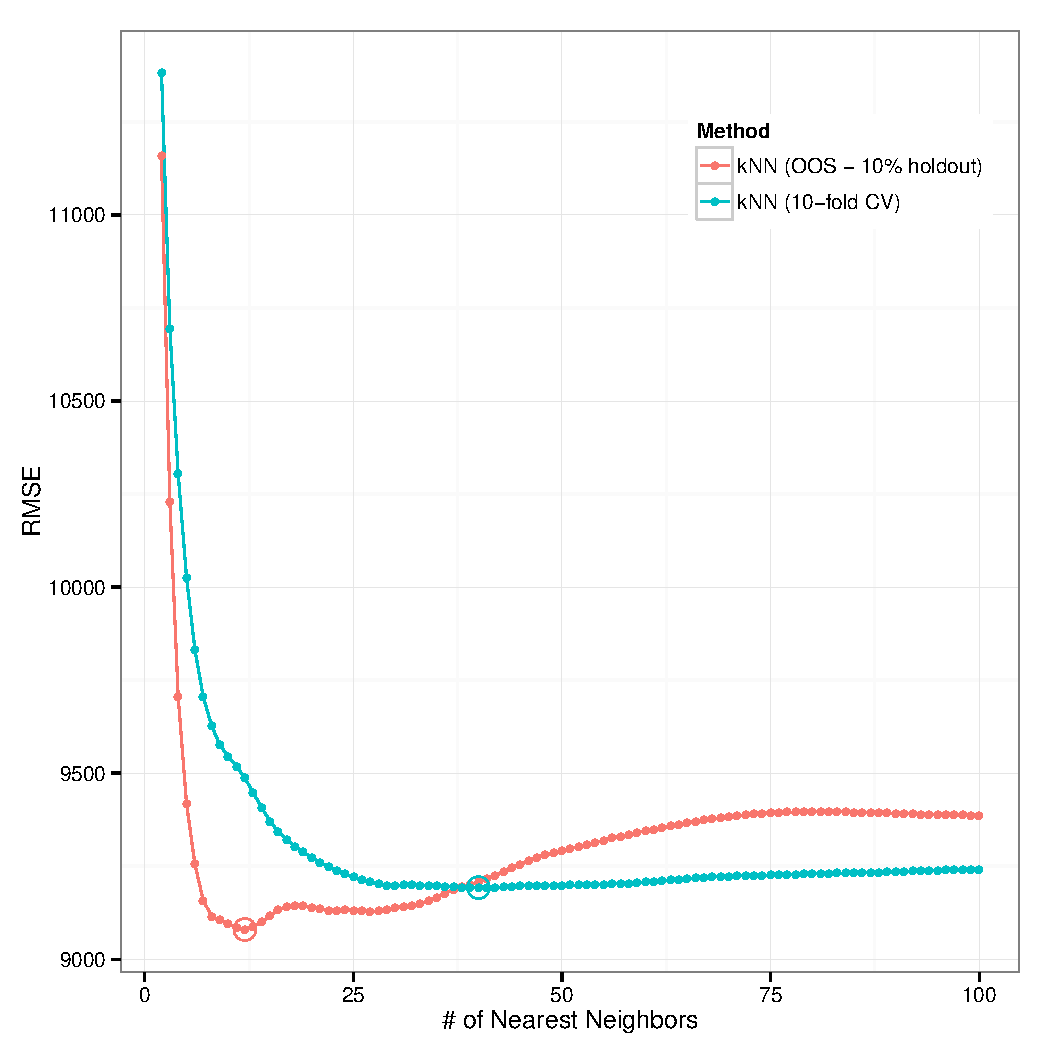
\includegraphics[scale=.5]{sweep_kknn.pdf}
  \caption{CV and OOS RMSE for Various Values of k in kNN}
  \label{fig:sweep}
\end{figure}

\section{Predictions}
% Predict car price with cross-validated knn and with linear model

\section{Appendix}

\begin{figure}[!htb]
  \centering
  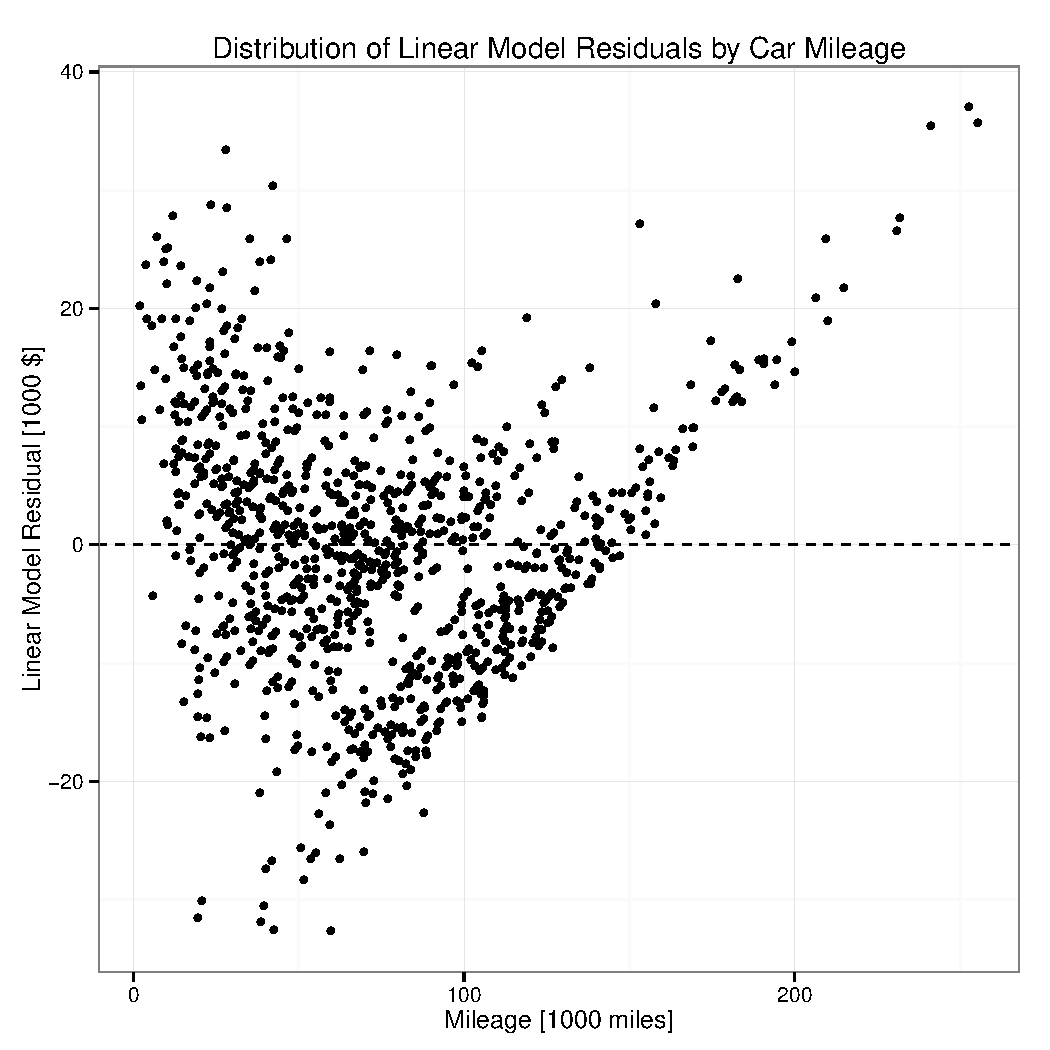
\includegraphics[scale=.5]{lin_errors.pdf}
  \caption{Distribution of Residuals in Linear Model}
  \label{fig:lin_errors}
\end{figure}

\end{document}

% \input{.tex}

% \begin{figure}
%   \centering
%   \begin{subfigure}[b]{0.49\textwidth}
%     \includegraphics[width=\textwidth]{.pdf}
%     \caption{}
%     \label{fig:}
%   \end{subfigure}
%   \hfill
%   \begin{subfigure}[b]{0.49\textwidth}
%     \includegraphics[width=\textwidth]{.pdf}
%     \caption{}
%     \label{fig:}
%   \end{subfigure}
%   \caption{}
% \end{figure}

% \begin{figure}[!htb]
%   \centering
%   \includegraphics[scale=.5]{.pdf}
%   \caption{}
%   \label{fig:}
% \end{figure}

